\documentclass{beamer}
\usepackage[utf8]{inputenc}
\usepackage[romanian]{babel}
\usepackage{hyperref}
\usepackage{mathtools}
\usepackage{listings}
\usepackage{graphicx}
\usepackage{float}
\usepackage{xcolor}
\usepackage{adjustbox}
\usepackage{scalerel}
\usepackage{tikz}
\usetikzlibrary{arrows}
\usetikzlibrary{calc}
\usepackage{pgfplots}

\setbeamercovered{transparent}
\usetheme{Madrid}
\title{Traffic Manager}
\author{Student: Mihai Andrei Gherghinescu \\ Supervizor: Lect. Dr. Todor Ivașcu}

\graphicspath{ {./images/} }

\begin{document}

\frame{\titlepage}

\section{Introducere}
    \begin{frame}{Introducere}
        Una dintre principalele cauze ale congestiilor in trafic
        sunt intersectiile. Acest fenomen este in special observat in 
        zonele urbane unde prezenta acestora este abundenta. 
        Pentru a minimiza timpul pierdut atat cat si siguranta soferilor 
        au fost dezvoltate sisteme de trafic inteligente(ITS). Acest 
        concept a fost reinventat dealungul timpului iar in prezent 
        este cuprins in notiunea de "smart city". Urmeaza sa prezint un 
        scurt istoric al evolutiei ITS cat si sa 
        prezint contributia proprie prin prezentarea unui nou tip de sistem.
    \end{frame}

\section{Privire de ansamblu asupra tehnologiei dezvoltate}
    \begin{frame}{Privire de ansamblu asupra tehnologiei dezvoltate}
        Dealungul timpului au fost concepute numeroase abordari ale 
        gestionari traficului. Noi o sa prezentam unele dintre cele 
        mai recente abordari care au dovenit a aduce imbunatatiri asupra
        traficului:
        \begin{itemize}[<+-| alert@+>]
            \item Sisteme bazate pe detectia de obiecte 
            \item Sisteme bazate pe senzori
            \item Sisteme care sincronizeaza traficul
            \item Sisteme bazate pe logica fuzzy
            \item Sisteme bazate pe DSRC
            
        \end{itemize}
    \end{frame}

    \begin{frame}{Sisteme bazate pe detectia de obiecte }
        \indent
        Sistemele se bazeaza pe determinarea numarul de masini ce 
        asteapta in trafic folosind camere (Fig ~\ref{fig:ObjectRecognitionSystem}).
        Metoda se bazeaza pe algoritmi de segmentare a imaginilor si detectie de obiecte.\\
        Cu toate acestea, tehnicile folosite pentru a rezolva
        problema s-au dovedit a fi ineficiente în timp real, datorita 
        complexitati computationale a algoritmilor de procesare a 
        imaginilor, astfel sistemul nu a putut tine pasul cu vehiculele 
        ce se deplasau la viteze mari. De asemnea, in conditii meteo 
        neprielnice, acuratetea acestora scade drastic.
        
    \end{frame}

    \begin{frame}{Sisteme bazate pe detectia de obiecte }
        \begin{figure}[h!]
            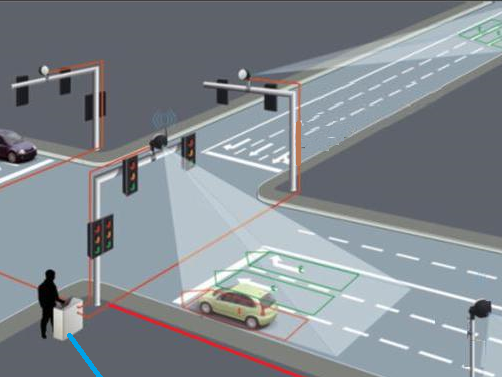
\includegraphics[width=(\textwidth / 4) * 3]{ObjectRecognitionSystemRepresentation.png}
            \caption{Sisteme bazate pe detectie de obiecte  
            (\href{https://english.mathrubhumi.com/news/kerala/knowing-traffic-camera-locations-isn-t-enough-to-escape-from-them-mvd-can-move-them-easily-1.7427787}{Sursa imagine} \textcopyright)}
            \label{fig:ObjectRecognitionSystem}
        \end{figure}

    \end{frame}

    \begin{frame}{Sisteme bazate pe senzori}
        O alta modalitate de a gestiona traficul este accea bazate pe senzori. 
        Aceasta presupune monitorizarea sosiri si plecari vehiculelor prin 
        intermediul datelor GPS.
        Astfel, am putea folosi tehnologia încorporată pentru a înregistra datele GPS și a le trimite
        la sistemul de monitorizare a traficului prin GSM/GPRS (Fig ~\ref{fig:SensorRecognitionSystem}). \\
        Dezavantajele acestei metode sunt faptul că implică costuri de implementare foarte mari, iar
        unele vehicule nu pot fi urmărite folosind sisteme de detectare radio.
        Această problemă poate fi abordata și cu ajutorul senzorilor de drum, dar ar necesita
        costuri chiar mai mari deoarece acestia ar trebui inlocuiti destul de des, 
        datorita uzuri parti carosabile si a constructiilor.
    \end{frame}

    \begin{frame}{Sisteme bazate pe senzori}
        \begin{figure}[h!]
            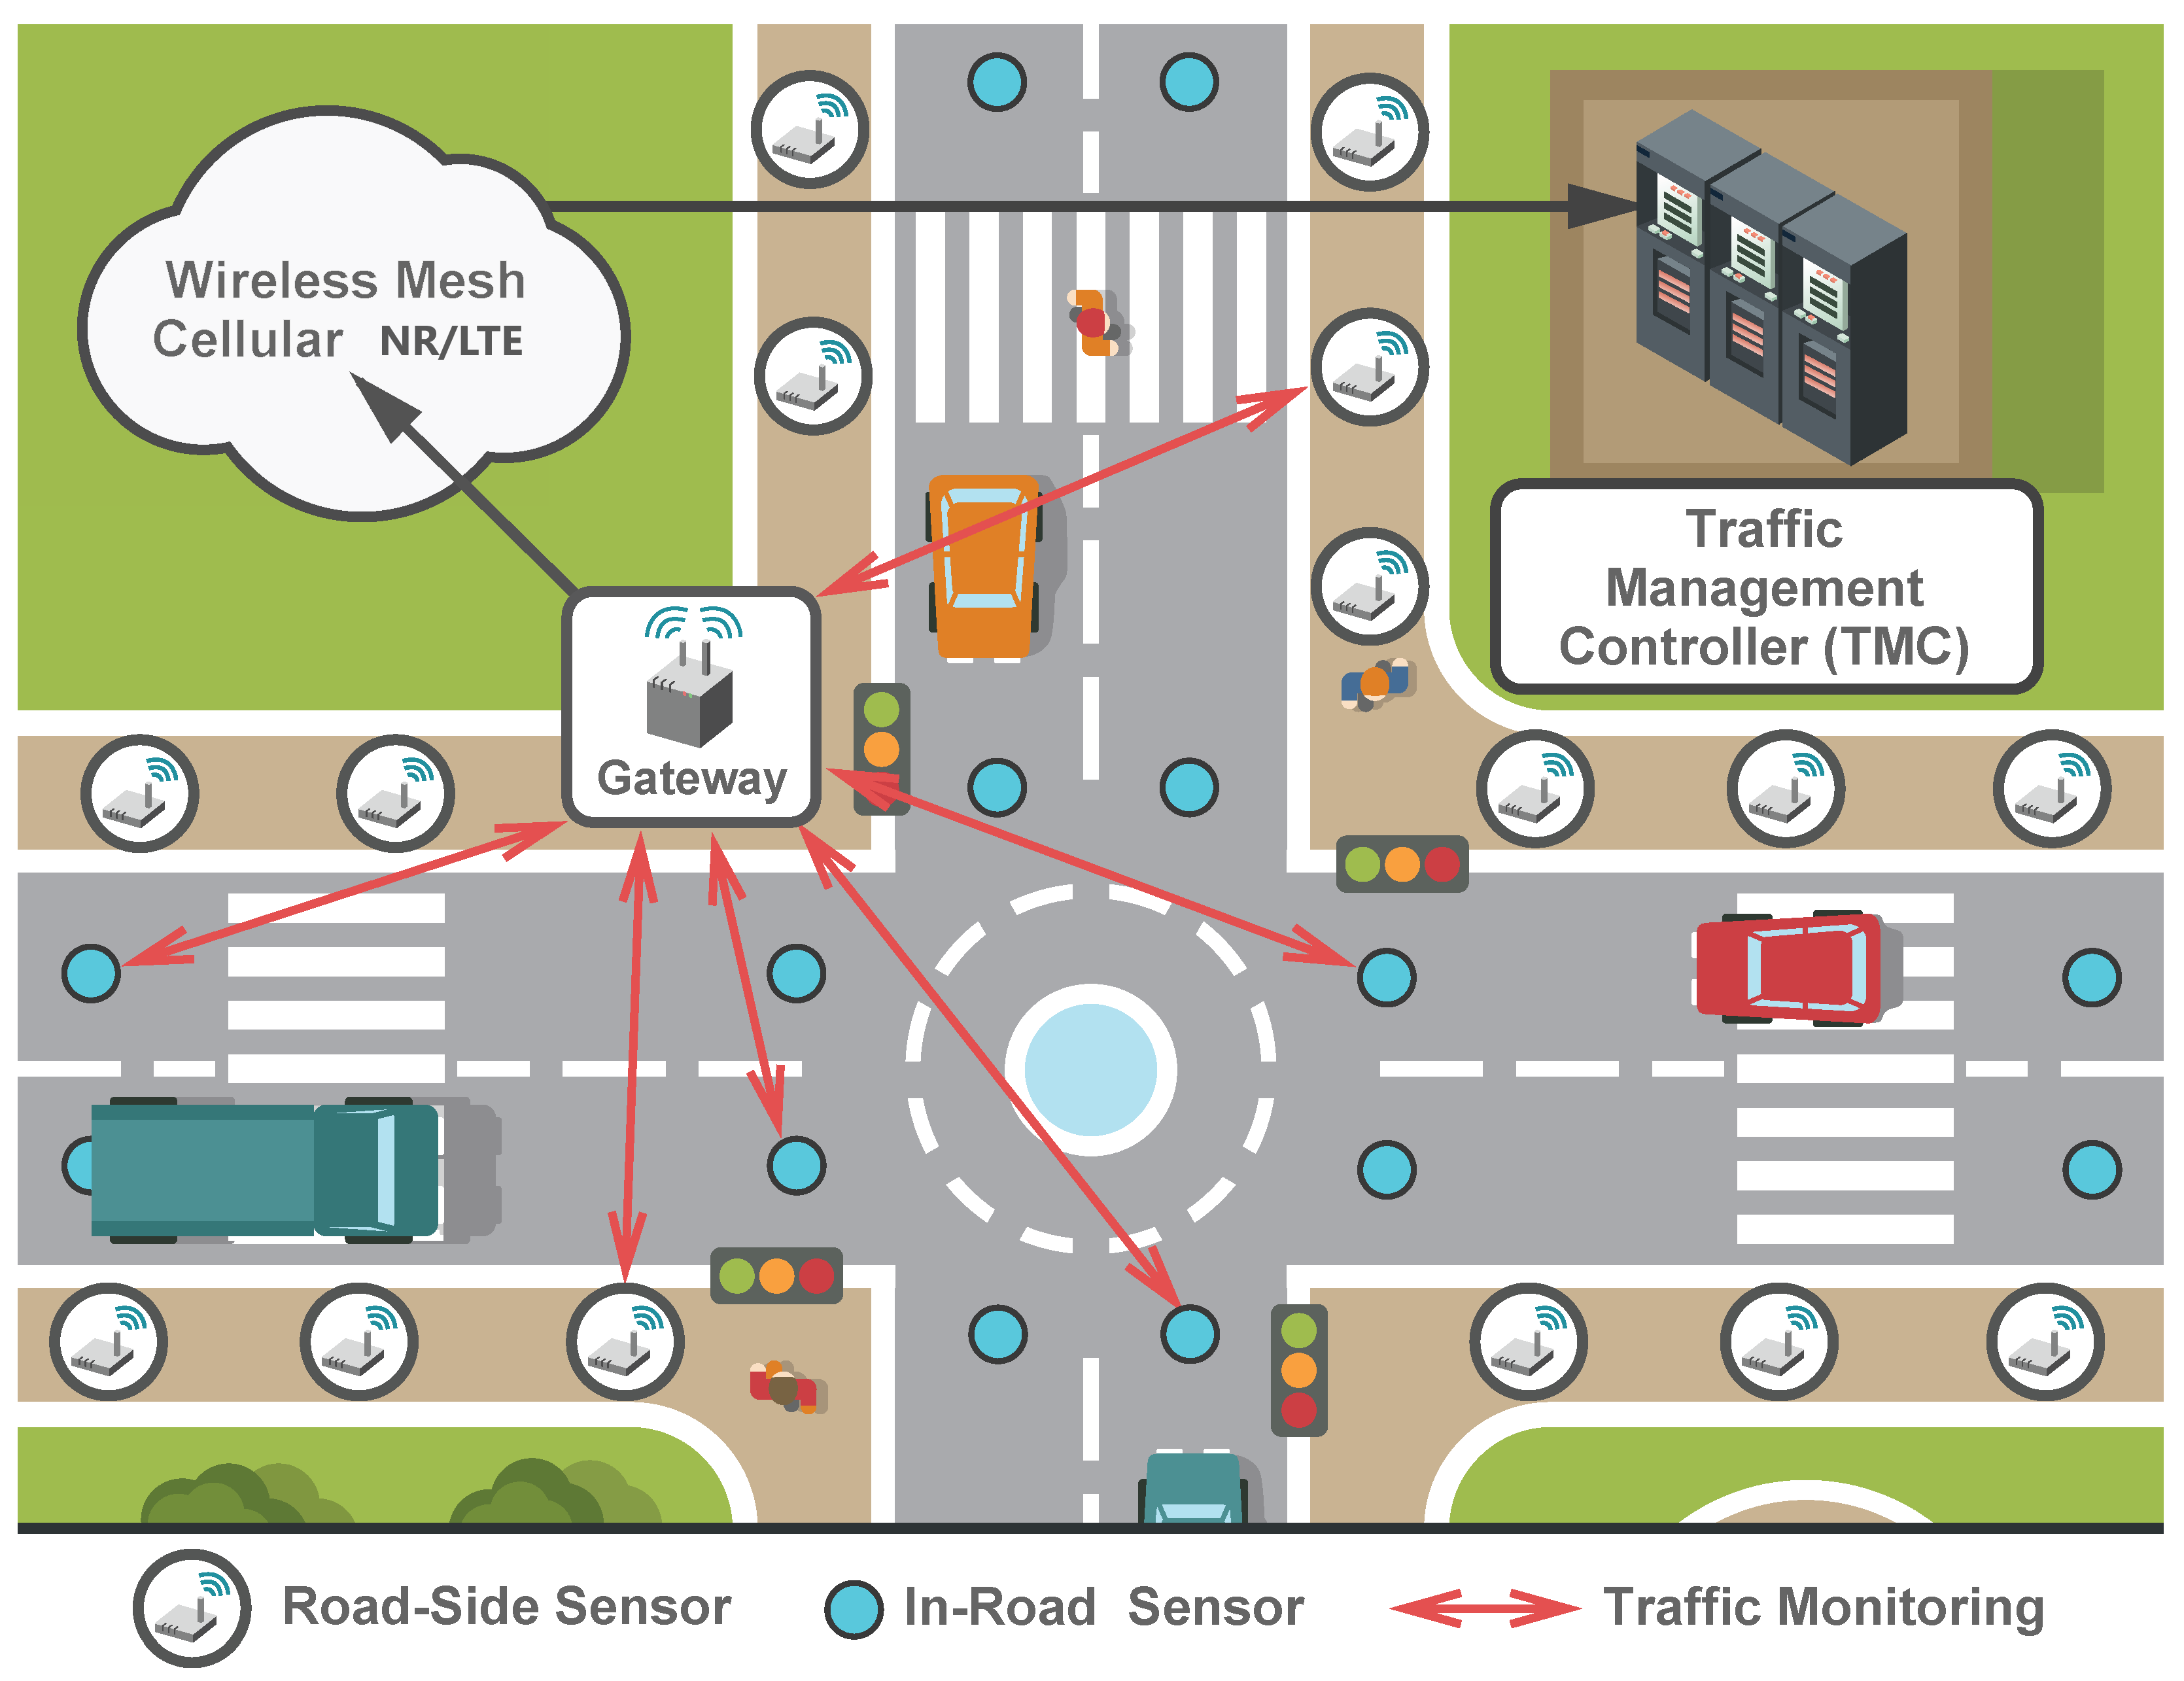
\includegraphics[width=(\textwidth / 4) * 3]{SensorsBasedTrafficControlSystemRepresentation.png}
            \caption{Sisteme bazate pe senzori 
            (\href{https://www.researchgate.net/figure/Communications-chain-of-data-feeds-in-smart-transportation_fig3_309740417}{Sursa imagine} \textcopyright)}
            \label{fig:SensorRecognitionSystem}
        \end{figure}
    \end{frame}

    \begin{frame}{Sisteme care sincronizeaza traficul}
        Sistemele de sincronizare a semafoarelor (TSC) urmăresc să minimizeze
        numărul de apariții STOP și GO prin adaptarea stari semafoarelor in intersectii.
        Această tehnică are ca si constrangere deplasarea la viteza constanta a vehiculelor,
        dand posibilitatea acestora sa treaca prin un lant de intersectii fara 
        oprire. La fel ca majoritatea altor metode, aceasta metoda colecteaza 
        date despre traficul curent, nefiind o anumita metoda specifica. 
        Cand vehiculele parcurg una dintre intersectii durata de verde creste, 
        la fel si cea de rosu pentru drumurile adiacente, dand posibilitatea curgeri 
        constante a traficului. \\
        Principalele dezavantaje ale acestei metode este ca in scenarii reale 
        conducatori nu vor respecta conditia de deplasare constanta in normele 
        legale de viteza, ducand la scenarii neprevazute, precum asteptarea 
        prelungita a rutelor secundare. De asemenea, metoda presupune prioritizarea 
        unei rute principale, in cazul in care doua sau mai multe rute principale 
        se intersecteaza traficul va fi desincronizat.

    \end{frame}

    \begin{frame}{Sisteme bazate pe logica fuzzy}
        Sistemele bazate pe logica fuzzy(FITS) au fost concepute initial 
        cu intentia de a imita un politist ce gestioneaza traficul dintr-o 
        intersectie. Acestea iau starea traficului si aplica reguli fuzzy 
        pentru a gestiona traficul. Astfel, starea traficului va fi 
        reprezentata de valori intra 0 si 1. De exemplu, durata timpului de 
        verde poate fi modelata pe baza setului fuzzy care include 4 stari:
        "none"(1), "scurt"(2), "moderat"(3), "lung"(4). \\
        In ciuda beneficiilor acestei abordari, asemnea altor algoritmi pe baza 
        de inteligenta artificiala, acesta necesita o perioada indelungata de 
        training, acesta facanduse real-time daturita faptului ca traficul este 
        mult prea variadic si nu poate fi prezis. De asemenea, acest 
        training va trebui realizat pentru fiecare intersectie in parte, iar 
        rezultatele nu coincide intodeauna cu asteptarile, traficul putand 
        chiar fi ingreunat din cauza algoritmului.
    \end{frame}

    \begin{frame}{Sisteme bazate pe logica fuzzy}
        \begin{equation}
            "none" - f(q) = max(min((10 - q) / 10, 2), 0)
        \end{equation}
        
        \begin{equation}
            "scurt" - f(q) = max(min(q / 10, (20 - q) / 10), 0)
        \end{equation}
        
        \begin{equation}
            "moderat" - f(q) = max(min(q / 5, (30 - q) / 5), 0)
        \end{equation}
        
        \begin{equation}
            "lung" - f(q) = max(min((50 - q) / 10, q / 2), 0)
        \end{equation}
    \end{frame}

    \begin{frame}{Sisteme bazate pe DSRC}
        DSRC sunt canale de comunicație fără fir unidirecționale sau
        bidirecționale special concepute pentru utilizare în automobile,
        care sunt utilizate în cea mai mare parte de către ITS pentru a
        comunica cu alte vehicule sau cu tehnologia infrastructurii.
        Acestea funcționează pe banda de 5,9 GHz a spectrului de frecvențe
        radio și sunt eficiente pe distanțe scurte si medii.
        Vitual Traffic Light(VTL) este o abordare inspirata din biologie 
        a controlului traficului care se bazeaza pe comunicare intre 
        vehicule (V2V) print utilizarea mesajelor DSRC.
        Ne putem imagina masinile ca fiind "routere in miscare", iar 
        intersectiile fiind "routere stationare". Ori de cate ori o 
        cale de transport este supraincarcata, una dintre rutele alternative 
        este blocata, astfel abordarea seamana mult cu tehnicile provenite 
        din retelistica.\\
        Principalul dezavantaj este faptul ca in momentul de fata sunt 
        multe vehicule care nu suporta acest tip de tehnologie. Astfel 
        infrastructura traficului nu permite in momentul de fata o lansare 
        a sistemului.
    \end{frame}

    \begin{frame}{Sisteme bazate pe DSRC}
        \begin{figure}[h!]
            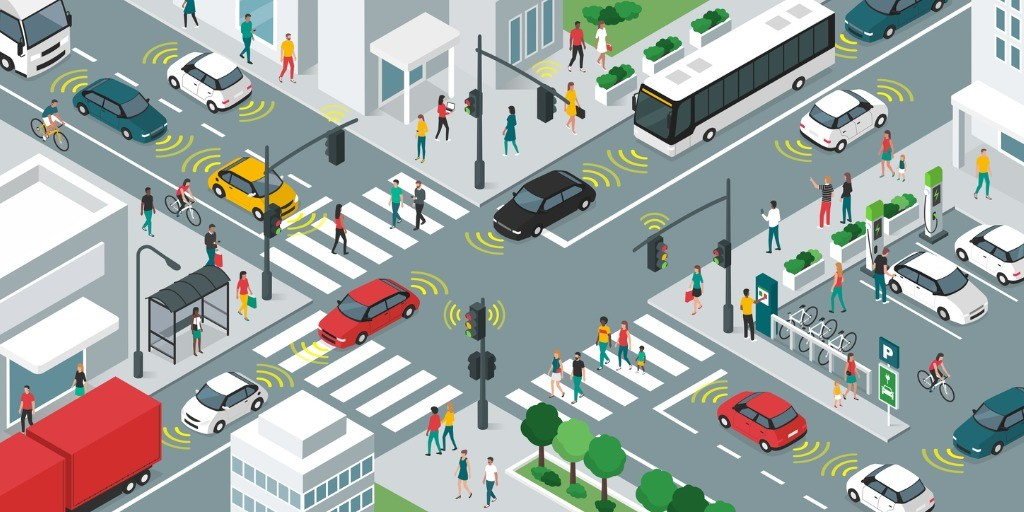
\includegraphics[width=\textwidth]{DSRCSystemModel.jpg}
            \caption{Sisteme bazate pe DSRC 
            (\href{https://www.frost.com/frost-perspectives/what-is-required-for-a-scalable-and-industry-wide-vehicle-to-everything-v2x-deployment/}{Sursa imagine} \textcopyright)}
            \label{fig:DSRCSystemModel}
        \end{figure}
        
    \end{frame}

\section{Motivatie, scopuri si obiective}
    \begin{frame}{Motivatie, scopuri si obiective}
        Ce ne-a determinat pe noi sa concepem acest nou tip de sistem este
        experienta in traficul Timisoara, Romania. 
        Credem că sistemul de trafic de aici se bazează pe sisteme de sincronizare a semafoarelor,
        deoarece de cele mai multe ori, atunci când puteți prinde semaforul
        verde la un anumita intersecție, le veti prinde si pe restul ce urmeaza.
        Ce este problematic si credem ca asta problema principala a soferilor 
        sunt orele de varf, cand traficul nu este gestionat bine si de 
        multe ori va trebuie sa astepti la acelasi semafor pana la 3 sau ba 
        chiar 4 cicluri de rosu si verde. Problema prezentata este datorita faptului 
        ca din cauza volumului mare de trafic, masinile nu vor mai putea circula 
        cu o viteza constanta iar traficul in sine va fi desincronizat.
        Acesta este doar un exemplu de trafic gestionat prost, dar 
        acesta problema persista la nivel global, netinand cont de 
        tipul de sistem folosit, mereu vom ajunge la ambuteiaje. 
        Principalele noastre obiective sunt crearea unui sistem:

        \begin{itemize}[<+-| alert@+>]
            \item Performant si accesibil
            \item Adaptabil la orice conditie de trafic
            \item Scalabil la nivel global
            
        \end{itemize}

    \end{frame}

\section{O noua varianta flexibila si economica de a gestiona traficul}
    \begin{frame}{O noua varianta flexibila si economica de a gestiona traficul}
        Credem că viitorul gestionari traficului se va baza pe semnale
        asemanatoare cu cele DSRC. Deocamdată, infrastructura nu oferă o
        modalitate de a implementa acest tip de sisteme, asa ca am decis
        să dezvoltăm o nouă abordare care să combină și să preia cele mai
        bune caracteristici din toate tehnologiile descrise mai sus și să
        ofere o migrare ușoară. Pentru asta am conceput un sistem IPC 
        alcatuit din 2 tipuri de servere si 2 tipuri de clienti:
        \begin{itemize}[<+-| alert@+>]
            \item Servere: 
            \begin{enumerate}
                \item  Junction Main Server(JMS) - legat de intersectie si semafoare
                \item  Proxy - servere regionale ce asigura conectivitatea
            \end{enumerate}
            \item Clienti:
            \begin{enumerate}
                \item Traffic Observer(TO) - legat de catre o camera pe fiecare directie
                \item Vehicle Tracker(VT) - instalat direct pe autovehicul
            \end{enumerate}
        \end{itemize}

    \end{frame}

    \begin{frame}{Vehicle tracker}
        Clientul respectiv se va folosi de componentele deja instalate 
        pe o masina anume: GPS si Radio. Astfel acesta va determina 
        pozitia geografica atat cat si directia de mers si prin
        intermediul Proxy-ului se va conecta la urmatoarea intersectie, 
        semnaland intentia de traversare. Odata ce clientul respectiv 
        a trecut de intersectie, el se va deconecta si va interoga 
        ultimul proxy cunoscut. Astfel, vom avea o metoda rapida si 
        neperturbabila de a transmite date catre semafor, putand determina 
        usor starea traficului in orice momemnt.
    \end{frame}

    \begin{frame}{Proxy}
    
    \end{frame}

    \begin{frame}{Traffic observer}
    
    \end{frame}

    \begin{frame}{Junction main server}
    
    \end{frame}

\section{Detalii de implementare}
    \begin{frame}{Detalii de implementare}

    \end{frame}

    \begin{frame}{Common}
        
    \end{frame}

    \begin{frame}{IPC}
        
    \end{frame}

    \begin{frame}{Car Detector}
        
    \end{frame}

    \begin{frame}{Object Recognition Server}
        
    \end{frame}

    \begin{frame}{Testing}
        
    \end{frame}

\section{Concluzii, defecte ale sistemului si directii viitoare}
    \begin{frame}{Concluzii, defecte ale sistemului si directii viitoare}

    \end{frame}
\end{document}